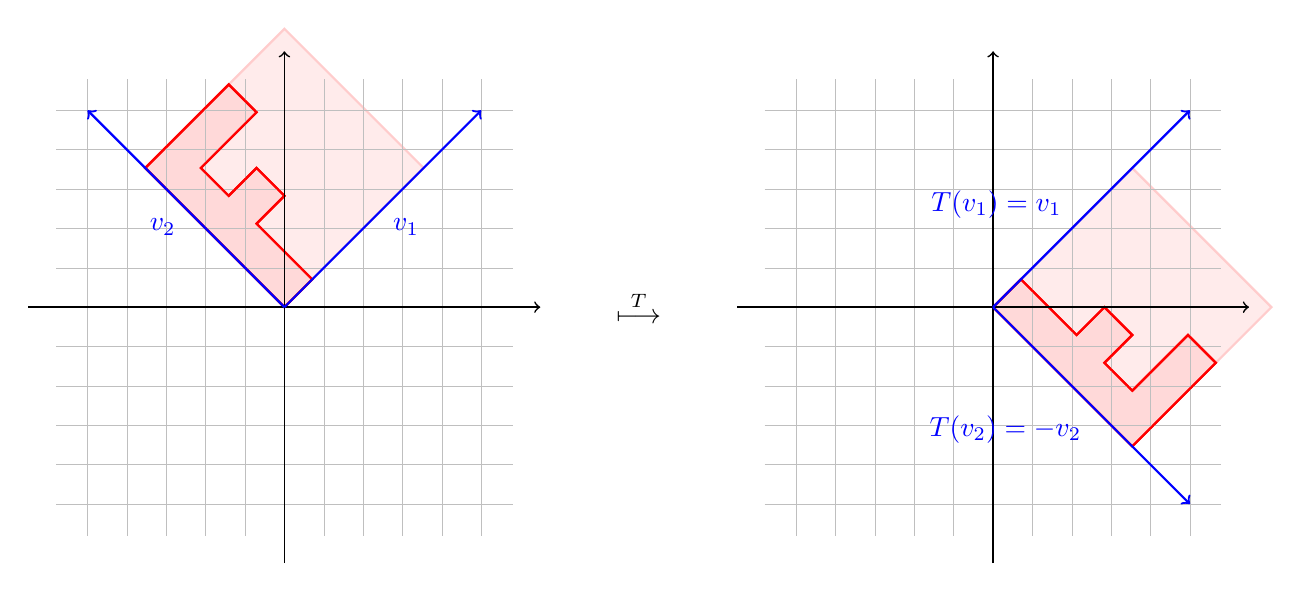
\begin{tikzpicture}
      \begin{scope}[scale=0.5]
        \draw[red!20,thick,fill=red!8,rotate=45]
        (0,0) -- (0,5) -- (5,5) -- (5,0) -- cycle;
        \draw[red,thick,fill=red!15,rotate=45]
        (0,0) -- (0,5) -- (3,5) -- (3,4) -- (1,4) --
        (1,3) -- (2,3) -- (2,2) -- (1,2) -- (1,0) -- cycle;
        \draw[step=1cm, gray!50, very thin] (-5.8,-5.8) grid (5.8,5.8);
        \draw[red,thick,rotate=45]
        (0,0) -- (0,5) -- (3,5) -- (3,4) -- (1,4) --
        (1,3) -- (2,3) -- (2,2) -- (1,2) -- (1,0) -- cycle;
        \draw[semithick,->] (-6.5,0) -- (6.5,0);
        \draw[semithick,->] (0,-6.5) -- (0,6.5);
        \draw[blue,thick,->] (0,0) -- node[below right] {$\vect{v}_1$} (5,5);
        \draw[blue,thick,->] (0,0) -- node[below left] {$\vect{v}_2$} (-5,5);
      \end{scope}
      \begin{scope}[xshift=4.5cm]
        \path (0,0) node {$\stackrel{T}{\longmapsto}$};
      \end{scope}
      \begin{scope}[xshift=9cm,scale=0.5]
        \draw[red!20,thick,fill=red!8,rotate=45,yscale=-1]
        (0,0) -- (0,5) -- (5,5) -- (5,0) -- cycle;
        \draw[red,thick,fill=red!15,rotate=45,yscale=-1]
        (0,0) -- (0,5) -- (3,5) -- (3,4) -- (1,4) --
        (1,3) -- (2,3) -- (2,2) -- (1,2) -- (1,0) -- cycle;
        \draw[step=1cm, gray!50, very thin] (-5.8,-5.8) grid (5.8,5.8);
        \draw[red,thick,rotate=45,yscale=-1]
        (0,0) -- (0,5) -- (3,5) -- (3,4) -- (1,4) --
        (1,3) -- (2,3) -- (2,2) -- (1,2) -- (1,0) -- cycle;
        \draw[semithick,->] (-6.5,0) -- (6.5,0);
        \draw[semithick,->] (0,-6.5) -- (0,6.5);
        \draw[blue,thick,->,cm={0,1,1,0,(0,0)}] (0,0) --
        node[above left,pos=0.4]
        {$T(\vect{v}_1) = \vect{v}_1$}
        (5,5);
        \draw[blue,thick,->,cm={0,1,1,0,(0,0)}] (0,0) --
        node[below left,pos=0.5]
        {$T(\vect{v}_2) = -\vect{v}_2$}
        (-5,5);
      \end{scope}
    \end{tikzpicture}
